% ========================================
% Chapter 5: Multi-Period Binomial Model and American Options
% ========================================
\chapter{Multi-Period Binomial Model and American Options}

\section{Multi-Period Binomial Model ($T=3$)}

Consider a binomial model with $T=3$ periods.  
The filtration is given by $(\mathcal{J}_t)_{t=0,\dots,3}$ with:
\[
\mathcal{J}_0=\{\emptyset,\Omega\},\quad
\mathcal{J}_1=\sigma(A_1,A_2),\quad
\mathcal{J}_2=\sigma(B_1,B_2,B_3,B_4),\quad
\mathcal{J}_3=\mathcal{P}(\Omega),
\]
where
\begin{itemize}
    \item $A_1 = \{\omega \in \Omega : \omega_1 = u\}$,
    \item $A_2 = \{\omega \in \Omega : \omega_1 = d\}$,
    \item $B_1 = \{\omega : \omega_1 = u,\ \omega_2 = u\}$,
    \item $B_2 = \{\omega : \omega_1 = u,\ \omega_2 = d\}$,
    \item $B_3 = \{\omega : \omega_1 = d,\ \omega_2 = u\}$,
    \item $B_4 = \{\omega : \omega_1 = d,\ \omega_2 = d\}$.
\end{itemize}

We consider a risk-free asset (bond) with price $S_t^0 = e^{rt}$  
and a risky asset (stock) with price $S_t^1$.

The evolution of the stock price can be represented by a binomial tree:

\begin{figure}[H]
\centering
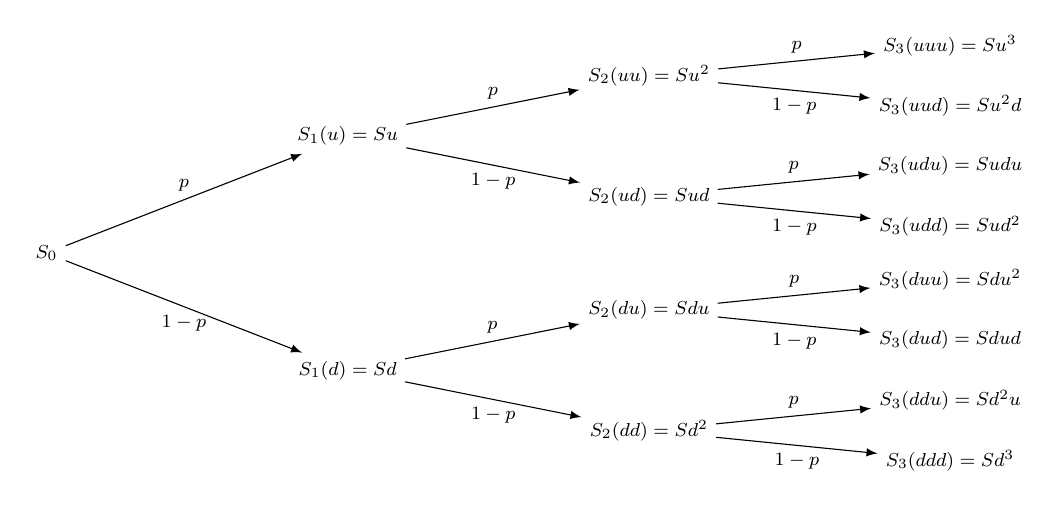
\begin{tikzpicture}[
    grow=right,
    scale=0.85, transform shape,
    level distance=45mm,
    level 1/.style={sibling distance=35mm},
    level 2/.style={sibling distance=18mm},
    level 3/.style={sibling distance=9mm},
    every node/.style={align=center, font=\footnotesize},
    edge from parent/.style={draw, -latex, thin},
    edge label/.style={font=\scriptsize, inner sep=1pt, sloped, above}
]

\node {$S_0$}
    child {
        node {$S_1(d)=Sd$}
        child {
            node {$S_2(dd)=Sd^2$}
            child {
                node {$S_3(ddd)=Sd^3$}
                edge from parent node[below] {$1-p$}
            }
            child {
                node {$S_3(ddu)=Sd^2u$}
                edge from parent node[above] {$p$}
            }
            edge from parent node[below] {$1-p$}
        }
        child {
            node {$S_2(du)=Sdu$}
            child {
                node {$S_3(dud)=Sdud$}
                edge from parent node[below] {$1-p$}
            }
            child {
                node {$S_3(duu)=Sdu^2$}
                edge from parent node[above] {$p$}
            }
            edge from parent node[above] {$p$}
        }
        edge from parent node[below] {$1-p$}
    }
    child {
        node {$S_1(u)=Su$}
        child {
            node {$S_2(ud)=Sud$}
            child {
                node {$S_3(udd)=Sud^2$}
                edge from parent node[below] {$1-p$}
            }
            child {
                node {$S_3(udu)=Sudu$}
                edge from parent node[above] {$p$}
            }
            edge from parent node[below] {$1-p$}
        }
        child {
            node {$S_2(uu)=Su^2$}
            child {
                node {$S_3(uud)=Su^2d$}
                edge from parent node[below] {$1-p$}
            }
            child {
                node {$S_3(uuu)=Su^3$}
                edge from parent node[above] {$p$}
            }
            edge from parent node[above] {$p$}
        }
        edge from parent node[above] {$p$}
    };
\end{tikzpicture}

\caption{Evolution of stock price in a 3-period binomial model.}
\end{figure}

\section{Absence of Arbitrage and Risk-Neutral Measure}

The no-arbitrage condition (NA) in the $T=3$ model is equivalent to its validity in each one-period sub-model.  
In the binomial case, it reads:
\begin{equation}
d < e^r < u.
\end{equation}

The existence of an equivalent martingale measure (EMM) $Q$ is equivalent to (NA).  
Under $Q$, the discounted stock price is a martingale:
\begin{equation}
\E_Q[\hat{S}_{t+1} \mid \mathcal{J}_t] = \hat{S}_t,
\end{equation}
where $\hat{S}_t = S_t / S_t^0 = e^{-rt} S_t$.

For any node $(\omega_1, \dots, \omega_t)$, we have:
\[
e^{-rt} S_t(\omega_1, \dots, \omega_t)
= \E_Q[e^{-r(t+1)} S_{t+1} \mid \mathcal{J}_t],
\]
that is:
\[
S_t = e^{-r} \left[ S_{t+1}(u)\, Q_{(\omega_1,\dots,\omega_t)}(u)
+ S_{t+1}(d)\, Q_{(\omega_1,\dots,\omega_t)}(d) \right].
\]

Let us solve for a particular node, for example $t=2$ after two up moves:
\[
S_2(uu) = e^{-r} \big[S_3(uuu)\, q_{uu} + S_3(uud)\,(1-q_{uu})\big],
\]
that is
\[
S u^2 = e^{-r} \big[S u^3 q_{uu} + S u^2 d (1-q_{uu})\big].
\]
We then obtain
\[
1 = e^{-r}\,[u q_{uu} + d(1-q_{uu})]
\quad\Rightarrow\quad
e^r = d + (u-d) q_{uu},
\]
hence the risk-neutral probability:
\[
q_{uu} = q = \frac{e^r - d}{u - d}, \qquad
1-q_{uu} = \frac{u - e^r}{u - d}.
\]
In this model, returns are path-independent, so the probability $q$ is the same at each node.

\section{Valuation and Hedging of a Contingent Claim}

To value a contingent claim with payoff $B$ at maturity $T=3$, we use the risk-neutral valuation formula:
\begin{equation}
A_t = \E_Q[B \mid \mathcal{J}_t],
\end{equation}
where $A_t$ denotes the claim price at date $t$.

To hedge the claim, we construct a self-financing portfolio $(H_t^0,H_t^1)$ such that its value coincides with the claim value at each date.  
The portfolio composition is given by:
\begin{align}
H_t^1 &= \frac{A_{t+1}(u) - A_{t+1}(d)}{S_{t+1}(u) - S_{t+1}(d)}
\quad &\text{(number of shares held)}\\
H_t^0 &= e^{-r}\,\big(A_{t+1}(u) - H_t^1 S_{t+1}(u)\big)
\quad &\text{(amount invested in risk-free asset).}
\end{align}
Since the market is complete, the measure $Q$ is unique and any claim can be perfectly replicated.

\section*{Numerical Example: Binomial Model}

Parameters: $T=3$, $u=1.1$, $d=0.9$, $r=\log(1+0.05)$, $S_0=20$

\subsection*{Stock Price Tree}

\begin{center}
\begin{tikzpicture}[scale=0.85, transform shape]
    % Node styles
    \tikzstyle{n} = [align=center, font=\small]
    
    % Nodes
    % t=0
    \node[n] (n0) at (0,0) {20};
    
    % t=1
    \node[n] (n1u) at (3, 1.5) {22 \\ \textcolor{red}{(20.95)}};
    \node[n] (n1d) at (3, -1.5) {18 \\ \textcolor{red}{(17.14)}};
    
    % t=2
    \node[n] (n2uu) at (6, 3) {24.2 \\ \textcolor{red}{(21.95)}};
    \node[n] (n2ud) at (6, 0) {19.8 \\ \textcolor{red}{(17.96)}};
    \node[n] (n2dd) at (6, -3) {16.2 \\ \textcolor{red}{(14.69)}};
    
    % t=3
    \node[n] (n3uuu) at (9, 4.5) {26.62 \\ \textcolor{red}{(23)}};
    \node[n] (n3uud) at (9, 1.5) {21.78 \\ \textcolor{red}{(18.81)}};
    \node[n] (n3udd) at (9, -1.5) {17.82 \\ \textcolor{red}{(15.39)}};
    \node[n] (n3ddd) at (9, -4.5) {14.58 \\ \textcolor{red}{(12.59)}};
    
    % Edges
    \draw[->] (n0) -- (n1u);
    \draw[->] (n0) -- (n1d);
    
    \draw[->] (n1u) -- (n2uu);
    \draw[->] (n1u) -- (n2ud);
    \draw[->] (n1d) -- (n2ud);
    \draw[->] (n1d) -- (n2dd);
    
    \draw[->] (n2uu) -- (n3uuu);
    \draw[->] (n2uu) -- (n3uud);
    \draw[->] (n2ud) -- (n3uud);
    \draw[->] (n2ud) -- (n3udd);
    \draw[->] (n2dd) -- (n3udd);
    \draw[->] (n2dd) -- (n3ddd);

\end{tikzpicture}
\end{center}

\vspace{1cm}

\noindent Notation: $\hat{S}_t$ and $\left(\hat{S}_t^1\right)$

\vspace{1cm}

\subsection*{Price of a European Put with $K=20$ and $T=3$}

$$\hat{B} = \left(-\hat{S}_T + K\right)_+ \quad \text{with} \quad K \cdot e^{-3r} \approx 17.28 \text{ (discounted strike value)}$$

\newpage

\subsection*{Risk-Neutral Probabilities}

Here $Q_{(w_1,w_2)}(w_u) = Q_{w_1}(w_u) = Q(w_u) = \frac{3}{4}$

$Q_{(w_1,w_2)}(w_d) = Q_{w_1}(w_d) = Q(w_d) = \frac{1}{4}$

\vspace{0.5cm}

$$B = \left(\frac{K}{e^{3r}} - S_3^1\right)_+ = A_3 = \begin{cases}
0 \\
0 \\
1.89 \\
4.69
\end{cases}$$

where $e^{3r} = 17.28$

\subsection*{Tree for $A_t$ (Option Price)}

The following binomial tree represents the European put option price at each node. Nodes are numbered from \circled{1} to \circled{6} and the discounted terminal payoff values ($A_3$) are indicated on the right.

\begin{center}
\begin{center}
\begin{tikzpicture}[scale=0.85, transform shape]
    % Node styles
    \tikzstyle{n} = [circle, draw, minimum size=0.9cm, font=\small, fill=white]
    \tikzstyle{l} = [font=\small, align=left]

    % Coordinates for Recombining Tree
    % t=0
    \node[n] (n1) at (0,0) {\circled{1}};
    
    % t=1
    \node[n] (n3) at (3, 1.5) {\circled{3}};
    \node[n] (n2) at (3, -1.5) {\circled{2}};
    
    % t=2
    \node[n] (n6) at (6, 3) {\circled{6}};
    \node[n] (n5) at (6, 0) {\circled{5}};
    \node[n] (n4) at (6, -3) {\circled{4}};
    
    % t=3 (Leaves/Payoffs)
    \node[right] at (8, 4.5) {0};
    \node[right] at (8, 1.5) {0};
    \node[right] at (8, -1.5) {1.89};
    \node[right] at (8, -4.5) {4.69};
    
    % Edges
    % t=0 -> t=1
    \draw[->, thick] (n1) -- (n3);
    \draw[->, thick] (n1) -- (n2);
    
    % t=1 -> t=2
    \draw[->, thick] (n3) -- (n6);
    \draw[->, thick] (n3) -- (n5);
    \draw[->, thick] (n2) -- (n5);
    \draw[->, thick] (n2) -- (n4);
    
    % t=2 -> t=3 (Payoff links)
    \draw[->] (n6) -- (7.5, 4.5);
    \draw[->] (n6) -- (7.5, 1.5);
    \draw[->] (n5) -- (7.5, 1.5);
    \draw[->] (n5) -- (7.5, -1.5);
    \draw[->] (n4) -- (7.5, -1.5);
    \draw[->] (n4) -- (7.5, -4.5);

\end{tikzpicture}
\end{center}
\end{center}

\begin{center}
\underline{Discounted Payoff}
\end{center}

\textbf{Backward Calculation of $A_t$:} We work backwards through the tree calculating the discounted expectation under $Q$ (with $q = 3/4$):

\begin{align*}
\circled{6} &= q \times 0 + (1-q) \times 0 = 0 \\
\circled{5} &= q \times 0 + (1-q) \times 1.89 \approx 0.47 \\
\circled{4} &= q \times 1.89 + (1-q) \times 4.69 \approx 2.58 \\[1em]
\circled{3} &= q \times \circled{6} + (1-q) \times \circled{5} \approx 0.12 \\
\circled{2} &= q \times \circled{5} + (1-q) \times \circled{4} \approx 1.00 \\[1em]
\circled{1} &= q \times \circled{3} + (1-q) \times \circled{2} \approx 0.34
\end{align*}

\newpage

\subsection*{Tree for $\textcolor{teal}{H_t^0}$ and $\textcolor{red}{H_t^1}$}

The following tree shows the hedging strategy values at each node. The \textcolor{teal}{teal} nodes represent $H^0$ (risk-free asset position) and the \textcolor{red}{red} nodes represent $H^1$ (Delta, risky asset position).

\begin{center}
\begin{center}
\begin{center}
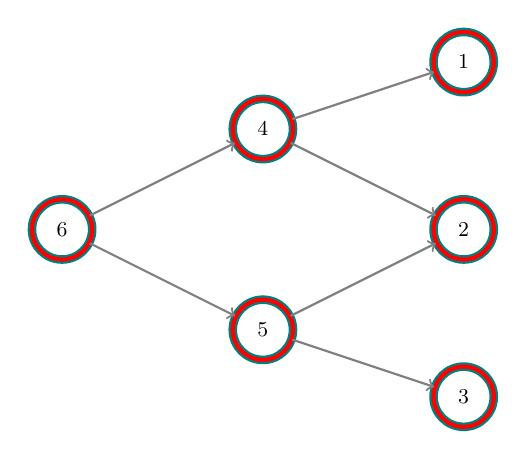
\begin{tikzpicture}[scale=0.85, transform shape]
    % Node styles
    % Double circle to represent both H^0 (teal) and H^1 (red)
    \tikzstyle{n} = [circle, draw=teal, double=red, double distance=1.5pt, minimum size=0.9cm, font=\small, fill=white, thick]
    
    % Tree Layout (Non-recombining for Strategy as per notes)
    % t=0
    \node[n] (n6) at (0,0) {\circled{6}};
    
    % t=1
    \node[n] (n4) at (3, 1.5) {\circled{4}};
    \node[n] (n5) at (3, -1.5) {\circled{5}};
    
    % t=2
    \node[n] (n1) at (6, 2.5) {\circled{1}}; % UU
    \node[n] (n2) at (6, 0) {\circled{2}}; % UD/DU (Recombining)
    \node[n] (n3) at (6, -2.5) {\circled{3}}; % DD
    
    % Edges
    \draw[->, thick, gray] (n6) -- (n4);
    \draw[->, thick, gray] (n6) -- (n5);
    
    \draw[->, thick, gray] (n4) -- (n1);
    \draw[->, thick, gray] (n4) -- (n2);
    
    \draw[->, thick, gray] (n5) -- (n2);
    \draw[->, thick, gray] (n5) -- (n3);

\end{tikzpicture}
\end{center}
\end{center}
\end{center}

\subsection*{For Example}

\textbf{Calculation of $H_2^1(w_u, w_u)$:}
\[
\circled{3} = H_2^1(w_u, w_u) = \frac{A_3(w_u, w_u, w_u) - A_3(w_u, w_u, w_d)}{S_3^1(w_u, w_u, w_u) - S_3^1(w_u, w_u, w_d)} = -1
\]

\textbf{Calculation of $H_2^0(w_u, w_u)$:} (financing asset)
\[
\circled{3} = H_2^0(w_u, w_u) = A_2(w_u, w_u) - H_2^1(w_u, w_u) \times S_2^1(w_u, w_u) = 17.27
\]

\subsection*{Similarly}

\begin{minipage}{0.45\textwidth}
\textbf{Values of $\textcolor{teal}{H^0}$:}
\begin{align*}
\textcolor{teal}{\circled{1}} &= 0 \\
\textcolor{teal}{\circled{2}} &= 10.35 \\
\textcolor{teal}{\circled{4}} &= 2.634 \\
\textcolor{teal}{\circled{5}} &= 11.95 \\
\textcolor{teal}{\circled{6}} &= 4.44
\end{align*}
\end{minipage}
\hfill
\begin{minipage}{0.45\textwidth}
\textbf{Values of $\textcolor{red}{H^1}$:}
\begin{align*}
\textcolor{red}{\circled{1}} &= 0 \\
\textcolor{red}{\circled{2}} &= -0.55 \\
\textcolor{red}{\circled{3}} &= -1 \\
\textcolor{red}{\circled{4}} &= -0.12 \\
\textcolor{red}{\circled{5}} &= -0.64 \\
\textcolor{red}{\circled{6}} &= -0.23
\end{align*}
\end{minipage}

\section{American Options}

\subsection{Definition}

An American option is a non-negative stochastic process $(\hat{X}_t)_{t=0,\dots,T}$ adapted to the filtration $(\mathcal{J}_t)$, which the holder can exercise at any time $t\in\{0,\dots,T\}$ to receive the payment $\hat{X}_t$.

\begin{itemize}
    \item American call option: $\hat{X}_t = (S_t - K)_+$,
    \item American put option: $\hat{X}_t = (K - S_t)_+$.
\end{itemize}

In a complete market, one cannot perfectly replicate an American option by a static strategy, because the exercise date is random.

\subsection{Valuation by Backward Induction}

Let $(\hat{U}_t)_{t=0,\dots,T}$ be the price process of an American option.  
At maturity: $\hat{U}_T = \hat{X}_T$.  
At date $T-1$, the holder chooses between:
\begin{enumerate}
    \item exercising and receiving $\hat{X}_{T-1}$;
    \item not exercising and keeping an option worth
    $\E_Q[e^{-r}\hat{X}_T \mid \mathcal{J}_{T-1}]$.
\end{enumerate}
Thus:
\[
\hat{U}_{T-1} = \max\!\left(\hat{X}_{T-1},\, \E_Q[e^{-r}\hat{U}_T\mid\mathcal{J}_{T-1}]\right),
\]
and, by induction, for all $t<T$:
\[
\hat{U}_t = \max\!\left(\hat{X}_t,\, \E_Q[e^{-r}\hat{U}_{t+1}\mid\mathcal{J}_t]\right).
\]

Setting $U_t = e^{-rt}\hat{U}_t$ and $X_t = e^{-rt}\hat{X}_t$ (discounted values), we obtain:
\begin{equation}
U_t = \max\!\left(X_t,\, \E_Q[U_{t+1}\mid\mathcal{J}_t]\right).
\end{equation}

\begin{proposition}[Snell Envelope]
The discounted process $(U_t)$ is the smallest supermartingale under $Q$ dominating the process $(X_t)$.
\end{proposition}

\begin{proof}
The proof proceeds in two steps:
\begin{enumerate}
    \item \textbf{$U$ dominates $X$ and is a supermartingale:}
    By definition, $U_t = \max(X_t, \E_Q[U_{t+1}|\mathcal{J}_t])$.
    Therefore $U_t \ge X_t$ (dominance).
    Moreover, $U_t \ge \E_Q[U_{t+1}|\mathcal{J}_t]$ (supermartingale).
    
    \item \textbf{$U$ is the smallest:}
    Let $(Y_t)$ be another supermartingale dominating $(X_t)$.
    At $t=T$, $U_T = X_T \le Y_T$.
    Suppose by induction that $U_{t+1} \le Y_{t+1}$.
    Then, by the supermartingale property of $Y$:
    \[
    \E_Q[U_{t+1}|\mathcal{J}_t] \le \E_Q[Y_{t+1}|\mathcal{J}_t] \le Y_t.
    \]
    Moreover, by the dominance hypothesis, $X_t \le Y_t$.
    Consequently:
    \[
    U_t = \max(X_t, \E_Q[U_{t+1}|\mathcal{J}_t]) \le \max(Y_t, Y_t) = Y_t.
    \]
    Thus, $U_t \le Y_t$ for all $t$, which proves that $U$ is the smallest dominating supermartingale.
\end{enumerate}
\end{proof}

\begin{proposition}[Non-Optimality of Early Exercise for a Call]
If the risk-free rate is non-negative ($S_t^0$ increasing), it is never optimal to exercise an American call option on a non-dividend-paying stock before maturity.
\end{proposition}

\begin{proof}[Detailed Proof]
We seek to prove that it is never optimal to exercise an American call option before its maturity $T$, provided the interest rate $r$ is positive. We reason by contradiction.

\begin{enumerate}
    \item \textbf{Contradiction hypothesis:} Suppose there exists a time $t < T$ where exercise is optimal. This means that the value obtained by exercising immediately, $S_t - K$ (intrinsic value), is strictly greater than the expected value if one keeps the option, $\E_Q[e^{-r} \hat{U}_{t+1} \mid \mathcal{J}_t]$ (continuation value).
    \[
    S_t - K > \E_Q[e^{-r} \hat{U}_{t+1} \mid \mathcal{J}_t]
    \]
    
    \item \textbf{Lower bound on future value:} The future option value, $\hat{U}_{t+1}$, is always at least equal to its intrinsic exercise value $(S_{t+1} - K)_+$.
    \[
    \hat{U}_{t+1} \ge (S_{t+1} - K)_+ \ge S_{t+1} - K
    \]
    
    \item \textbf{Taking expectation:} Take the discounted conditional expectation of this inequality:
    \[
    \E_Q[e^{-r} \hat{U}_{t+1} \mid \mathcal{J}_t] \ge \E_Q[e^{-r} (S_{t+1} - K) \mid \mathcal{J}_t]
    \]
    
    \item \textbf{Martingale Property:} The right-hand term expands by linearity:
    \[
    \E_Q[e^{-r} S_{t+1} \mid \mathcal{J}_t] - e^{-r} K
    \]
    Under measure $Q$, the discounted price $e^{-rt} S_t$ is a martingale. Therefore $\E_Q[e^{-r(t+1)}S_{t+1} \mid \mathcal{J}_t] = e^{-rt}S_t$. Multiplying by $e^{rt}$, we have $\E_Q[e^{-r} S_{t+1} \mid \mathcal{J}_t] = S_t$.
    The inequality thus becomes:
    \[
    \E_Q[e^{-r} \hat{U}_{t+1} \mid \mathcal{J}_t] \ge S_t - e^{-r} K
    \]
    
    \item \textbf{Contradiction:} Combine the initial hypothesis (1) and result (4):
    \[
    S_t - K > \E_Q[e^{-r} \hat{U}_{t+1} \mid \mathcal{J}_t] \ge S_t - e^{-r} K
    \]
    Simplifying by $S_t$, we obtain:
    \[
    -K > -e^{-r} K
    \]
    Multiplying by $-1$ (which reverses the inequality):
    \[
    K < e^{-r} K \iff K(1 - e^{-r}) < 0
    \]
    Now, if $r > 0$, then $e^{-r} < 1$, so $(1 - e^{-r}) > 0$. Since $K > 0$ as well, the product $K(1 - e^{-r})$ is \textbf{strictly positive}, which contradicts the inequality $K(1 - e^{-r}) < 0$.
    
    This contradiction shows that the initial hypothesis is false: it is never optimal to exercise an American call prematurely.
\end{enumerate}
\end{proof}

\subsection{Numerical Example: American Put Option}
Let us revisit the same binomial model as before: $S_0=20, u=1.1, d=0.9, r=\ln(1.05)$, but with an American put option with strike $K=22$.

\begin{tcolorbox}[title=Decision Tree: Exercise or Wait?, colback=blue!5!white, colframe=blue!50!black]
Calculations are done backward. At each node, we compare the intrinsic value $K-S_t$ with the continuation value.
\begin{itemize}
    \item $\mathbf{t=3}$: Payoff $P_3 = (22 - S_3)_+$.
    \begin{itemize}
        \item $S_3(ddd) = 14.58 \implies P_3 = 7.42$
        \item $S_3(udd) = 17.82 \implies P_3 = 4.18$
        \item $S_3(uud) = 21.78 \implies P_3 = 0.22$
        \item $S_3(uuu) = 26.62 \implies P_3 = 0$
    \end{itemize}
    \item $\mathbf{t=2}$: $P_2 = \max(22-S_2, e^{-r}[q P_3(u) + (1-q) P_3(d)])$.
    \begin{itemize}
        \item Node $dd$ ($S_2=16.2$): Intrinsic $= 5.8$. Continuation $\approx 4.75$. $\to$ \textbf{Exercise} (value 5.8).
        \item Node $ud$ ($S_2=19.8$): Intrinsic $= 2.2$. Continuation $\approx 1.15$. $\to$ \textbf{Exercise} (value 2.2).
        \item Node $uu$ ($S_2=24.2$): Intrinsic $= 0$. Continuation $\approx 0$. $\to$ No exercise.
    \end{itemize}
    \item $\mathbf{t=1}$:
    \begin{itemize}
        \item Node $d$ ($S_1=18$): Intrinsic $= 4$. Continuation $\approx 2.95$. $\to$ \textbf{Exercise} (value 4).
        \item Node $u$ ($S_1=22$): Intrinsic $= 0$. Continuation $\approx 0.52$. $\to$ No exercise.
    \end{itemize}
    \item $\mathbf{t=0}$ ($S_0=20$): Intrinsic $= 2$. Continuation $\approx 1.32$. $\to$ \textbf{Immediate Exercise} (value 2).
\end{itemize}
\end{tcolorbox}
Conclusion: In this specific example, the American put option has a value of 2 (immediate exercise), significantly higher than the corresponding European option (which would be worth approximately 1.32). This illustrates the early exercise premium.

\section{Stopping Times and American Options}

\begin{definition}[Stopping Time]
A random variable $\tau : \Omega \to \{0,\dots,T\}$ is a \emph{stopping time} if,
for all $t$, the event $\{\tau = t\}$ belongs to $\mathcal{J}_t$.
\end{definition}

\paragraph*{Intuition: The Best Time to Act}
The problem of American option valuation is a canonical example of an "optimal stopping problem". The option holder faces a series of decisions: at each time $t$, should they exercise the option and collect the gain $X_t$, or should they wait hoping for a higher future gain? A "stopping time" $\tau$ is a decision rule that depends only on the past and present. The holder seeks the optimal stopping time $\tau^*$ that maximizes the expected discounted gain, i.e., $\max_\tau \E_Q[X_\tau]$.

The backward induction formula we established ($U_t = \max(X_t, \E_Q[U_{t+1} \mid \mathcal{J}_t])$) is none other than Bellman's dynamic programming algorithm that solves this optimal stopping problem. At each step, it compares the value of immediate action ("exercise now") with the expected value of the optimal future strategy ("continue and make the best decision later"). The process $U_t$ thus represents the maximum attainable value from time $t$ onward.

Exercising an American option amounts to choosing a stopping time $\tau$.  
The gain obtained is $X_\tau$.  
\begin{proof}
We must show that the process defined by $U_t = \sup_{\tau \in \mathcal{T}_t} \E_Q[X_\tau | \mathcal{J}_t]$ indeed satisfies Bellman's recurrence equation (Proposition 1).
Let $V_t$ be this supremum.
At $t=T$, $V_T = X_T = U_T$.
For $t < T$, separate the set of stopping times $\mathcal{T}_t$ into two cases: $\tau = t$ (immediate exercise) and $\tau > t$ (continuation).
If $\tau > t$, then $\tau$ is also a stopping time in $\mathcal{T}_{t+1}$.
\[
V_t = \max \left( X_t, \sup_{\tau \in \mathcal{T}_{t+1}} \E_Q[X_\tau | \mathcal{J}_t] \right)
\]
Using the tower property (law of iterated expectations):
\[
\E_Q[X_\tau | \mathcal{J}_t] = \E_Q [ \E_Q[X_\tau | \mathcal{J}_{t+1}] | \mathcal{J}_t ]
\]
Therefore:
\[
\sup_{\tau \in \mathcal{T}_{t+1}} \E_Q[X_\tau | \mathcal{J}_t] = \E_Q \left[ \sup_{\tau \in \mathcal{T}_{t+1}} \E_Q[X_\tau | \mathcal{J}_{t+1}] \mid \mathcal{J}_t \right] = \E_Q[V_{t+1} | \mathcal{J}_t]
\]
We thus recover:
\[
V_t = \max(X_t, \E_Q[V_{t+1} | \mathcal{J}_t])
\]
This is exactly the recurrence relation that defines $(U_t)$. By uniqueness, $U_t$ is indeed the supremum of expected gains over all possible stopping times.
\end{proof}
